\documentclass[60pt]{article}
% Formatting
\usepackage[utf8]{inputenc}
\usepackage[margin=1in]{geometry}
\usepackage[titletoc,title]{appendix}
\usepackage{amsmath,amsfonts,amssymb,mathtools}
\usepackage[normalem]{ulem}
\usepackage{graphicx,float}
\usepackage[ruled,vlined]{algorithm2e}
\usepackage{algorithmic}
\usepackage{makecell}
\usepackage{caption}
\usepackage{subcaption}
\usepackage{pdfpages}
\renewcommand\cellalign{lt}

\renewcommand{\baselinestretch}{1.5}
\def\tobar{\mathrel{\mkern8mu  \vcenter{\hbox{$\scriptscriptstyle+$}}%
                    \mkern-18mu{\longrightarrow}}}
\newcommand\ddfrac[2]{\frac{\displaystyle #1}{\displaystyle #2}}
\let\uglyepsilon\epsilon
\let\epsilon\varepsilon
\let\varepsilon\uglyepsilon
\usepackage{physics}
\usepackage{enumitem}
\usepackage{tabularx}
\usepackage{ebproof}
% Code syntax highlighting
% https://www.overleaf.com/learn/latex/Code_Highlighting_with_minted
\usepackage{minted}
\usemintedstyle{friendly}
\usepackage{hyperref}
\usepackage{xcolor}
\definecolor{LightGray}{gray}{0.9}
\setminted{
frame=lines,
framesep=2mm,
baselinestretch=1.2,
bgcolor=LightGray,
fontsize=\footnotesize,
linenos
}
\usepackage[parfill]{parskip}
\usepackage{listings}% http://ctan.org/pkg/listings
\lstset{
  basicstyle=\ttfamily,
  mathescape
}
\let\verbatim\someundefinedcommand
\lstnewenvironment{verbatim}
{}{}
% Title content
\title{Computer Science Tripos Part II Project Phase 3 Proposal}
\author{Thomas Yuan}

\begin{document}
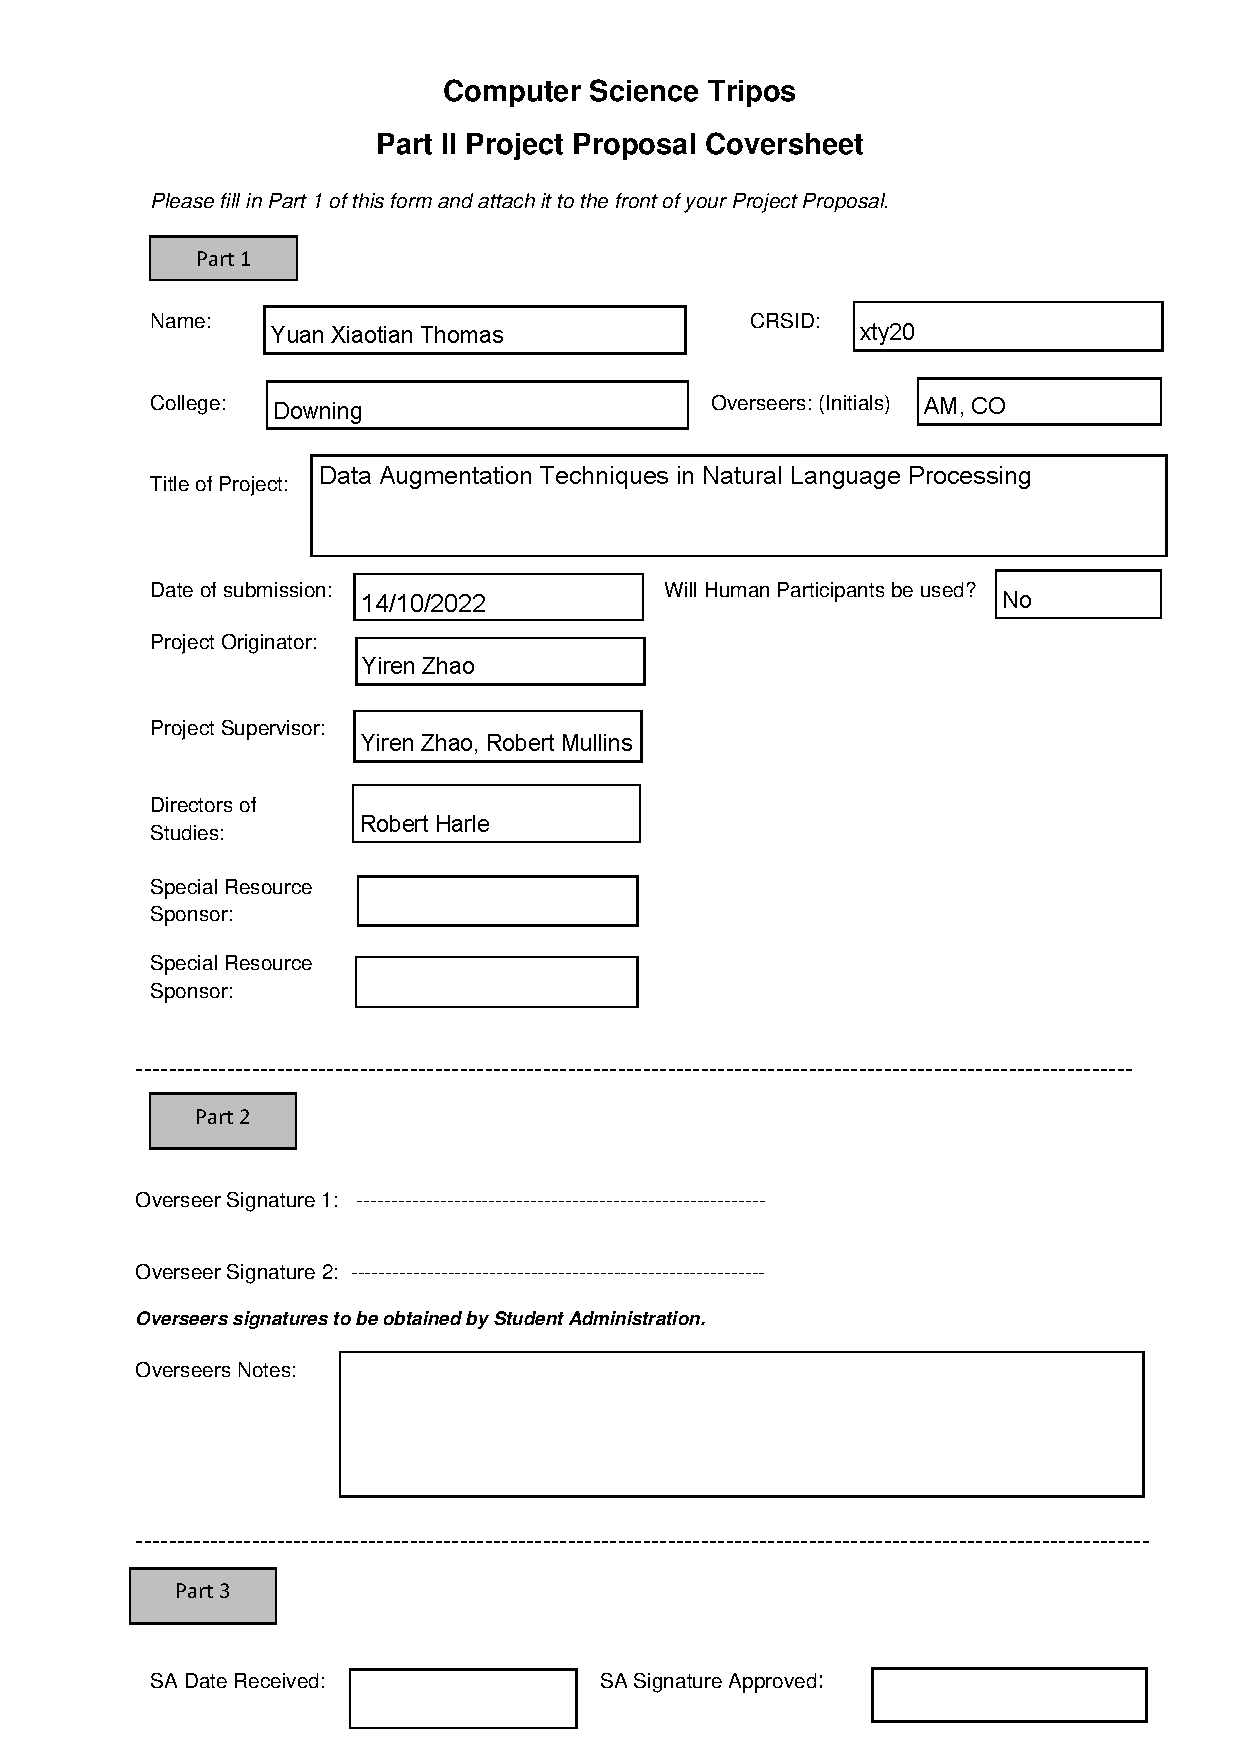
\includepdf{Thomas_Yuan_Project_Proposal_Cover_Sheet.pdf}
\maketitle
\begin{center}
\textbf{\Large Data Augmentation Techniques in Natural Language Processing}
\end{center}

\section{Introduction and Description}
\par
Data augmentation is a technique used in deep learning to increase the amount of data available for training, usually by modifying existing copies of data. By artificially generating more data points, data augmentation helps deal with the issue of limited or scarce data, improving the quality and quantity of the dataset such that the trained model is better and is less prone to overfitting. Some commonly used techniques include synonym replacement and back translation which uses a translation model to translate text to and from other languages in order to obtain syntactically different sentences. Other techniques such as insertion and deletion adds noise to the data by inserting and deleting words randomly.
\par
Data augmentation in natural language processing is more interesting than general deep learning tasks because of the nature of natural languages and how there are interesting rules to manipulate text such that the syntax is different, but the semantics are still the same, for example swapping words with their synonyms or changing the structure of the sentence. This results in new augmentation techniques, namely paraphrasing-based techniques apart from the usual noising and sampling-based techniques that utilize statistical properties to perform data augmentation. 
\par
Moreover, data augmentation has also been widely used in computer vision to help train models to perform tasks such as identifying objects in pictures, and some notable techniques in recent years include CutMix \cite{yun2019cutmix} and MixUp \cite{zhang2017mixup}. Therefore this project aims to explore data augmentation techniques in natural language processing tasks and see how they affect the performance of the trained model, especially under varying scarcities of data, as well as look into how specific data augmentation techniques in computer vision can be applied in natural language processing. 
\par

To achieve this, I will be training neural network models on the tasks text classification and seq2seq machine translation, and using data augmentation techniques including paraphrasing and noising-based ones. For each of these techniques, I will be applying them to the dataset, and training the model using this augmented dataset. Afterwards, I will be measuring the performance of the model, using accuracy in classifying texts for text classification and BLEU score \cite{papineni-etal-2002-bleu} for machine translation to evaluate the quality of the translation. I will compare the performance between these augmented datasets and also unaugmented datasets to see how these techniques affect the performance of the model.

\section{Starting Point}
\par
The external libraries that will be used for this project include open source library PyTorch, as well as sub-libraries torchtext and torchnlp. These libraries will be used to implement the neural network model and to help prepare datasets. During September 2022, I went through the PyTorch tutorial and learnt how to implement a basic neural network model to classify images, which was my first time using PyTorch. I have also read through some documentation of torchtext and torchnlp, but no code on NLP-specific neural network models has been written yet. This was also my first time reading into data augmentation, where I read through 3-4 papers on data augmentation linked to me by supervisors, including some surveys of techniques used in NLP. Before that, I had no prior experience with deep learning implementations or data augmentation.

\section{Substance and Structure of the Project}
\par
The project uses the following key concepts:
\par
\textbf{Seq2seq machine translation} Seq2seq is a machine learning approach commonly used in machine translation, which uses a recurrent neural network to transform one sequence into another sequence. In this project it will be implemented as an encoder and a decoder (along with some other components for optimization) transforming sequences of English words into German words.
\par
\textbf{CutMix} CutMix is a data augmentation technique used in computer vision, where it cuts out portions of images with different labels and pieces them together, with the label being a mix of the labels the original images have. \ref{fig:cutmix} This method aims to help the network learn about a wider range of features such that the trained model can generalize better.
\begin{figure}[!h]
    \centering
    \begin{subfigure}[t]{0.3\textwidth}
        \centering
        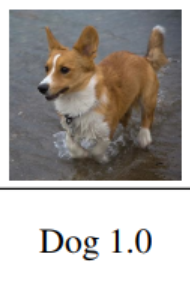
\includegraphics[width=0.6\textwidth]{dog.png}
        \caption{An image of a dog and its label.}
        \label{fig:dog}
    \end{subfigure}
    \hfill
    \begin{subfigure}[t]{0.3\textwidth}
        \centering
        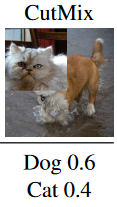
\includegraphics[width=0.6\textwidth]{cutmix.png}
        \caption{An image of the dog and a cat pieced together using the CutMix algorithm, with corresponding labels}
        \label{fig:cutmix}
    \end{subfigure}
    \hfill
    \begin{subfigure}[t]{0.3\textwidth}
        \centering
        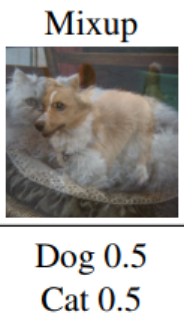
\includegraphics[width=0.6\textwidth]{mixup.png}
        \caption{An image of the dog and a cat mixed together using the MixUp algorithm, with corresponding labels.}
        \label{fig:mixup}
    \end{subfigure}
    \caption{Unaugmented and augmented dog images}
    \label{fig:dog images}
\end{figure}
\newpage
\par
\textbf{MixUp} MixUp is a data augmentation technique used in computer vision, where features and their labels are mixed together \ref{fig:mixup}. It is implemented using the following formula
\[\hat{x} = \lambda x_i + (1-\lambda)x_j, \quad \text{where }x_i,x_j \text{ are raw input vectors}\]
\[\hat{y} = \lambda y_i + (1-\lambda)y_j, \quad \text{where }y_i,y_j \text{ are one-hot label encodings}\]
As a result, neural networks become less prone to memorizing corrupt labels and networks are not overconfident about the correlation between features and labels.
\par
The project has the following main work items:
\par
\textbf{Preliminary Reading} I would have to perform some further reading on PyTorch, torchtext and torchnlp to become more familiar with them. I would also need to read more into the different augmentation methods and decide on how exactly I should implement them.
\par 

\textbf{Neural network models} I would have to implement a text classification model and a seq2seq English-to-German machine translation model.
\par

\textbf{Data augmentation techniques} I would have to implement synonym replacement, back translation, insertion and deletion. For extensions, I would have to implement these for German as well, and also I would have to implement CutMix and MixUp.
\par

\textbf{Training and Testing} I would have to train my networks on datasets, and implement performance measurements to measure the performance of my trained networks. For extensions, I would have to train my networks on larger datasets.
\par

\textbf{Dissertation} I will work on the dissertation throughout the project along with writing the code. I will finish the dissertation after writing the source code and performing all the training and testing required.

\section{Success Criterion}
\par 
In order to be considered a success, the project should have achieved the following:
\begin{enumerate}
    \item Implemented a neural network model for text classification, trained and tested on the AGNews \cite{Zhang2015CharacterlevelCN} corpus, measure accuracy and make comparison with other models that usually achieve 85-95\% accuracy
    \item Implemented a neural network model for seq2seq machine translation, trained and tested on the IWSLT \cite{cettolo-etal-2017-overview} dataset, measure BLEU score and make comparison with other models that usually achieve a BLEU score of 20-30
    \item Implemented data augmentation functions including synonym replacement, back translation, insertion and deletion
    \item Train and evaluate implemented network models using augmented datasets and evaluating performance using accuracy for text classification and BLEU score for machine translation
    \item Evaluate the effectiveness of data augmentation techniques with accuracy and BLEU score using p-tests
    
\end{enumerate}
\section{Extensions}
\par
Some potential extensions for the project include:
\begin{enumerate}
    \item Use a larger dataset (WMT'16 \cite{bojar-EtAl:2016:WMT1}) for training and testing the models, evaluate performance of models using above-mentioned performance metrics
    \item Augment both target and source text in translation text using the same data augmentation techniques but for German
    \item Implement CutMix and MixUp and evaluate performance of models trained using these augmentation techniques
\end{enumerate}

\section{Timetable and Planning of Work}
\par
I have broken down my workload into 15 work items, including 2 breaks, each of which should last around 2 weeks. I have included a description of each of these work items, the weeks they span, and some milestones that should be completed by the end of that particular work item.

\begin{tabularx}{\textwidth}{|X|X|X|}
    \hline
    Date & 
    Description & 
    Milestones 
    \\ \hline
    1. 17/10 - 30/10 & 
    - Familiarize myself with PyTorch, torchtext and torchnlp \newline
    - Do more reading and research into how NLP tasks are implemented \newline
    - Implement a neural network model for text classification and Seq2Seq machine translation & 
    Finished implementing the two models and tested that they work according to expected using small training datasets 
    \\ \hline 
    2. 31/10 - 13/11 & 
    - Implement data preparation and preprocessing functions such that the datasets can be used for augmentation and models \newline
    - Read more into the various augmentation methods, specifically back-translation as well as MixUp, figure out exact implementation details including what libraries and algorithms to use \newline
    - Implement synonym replacement and back-translation (augmentation techniques) &
    - Finished implementing the two mentioned augmentation techniques, tested that they work according to expected on data \newline
    - Finished preparing datasets
    \\ \hline 
    3. 14/11 - 27/11 & 
    - Implement insertion and deletion (augmentation techniques) \newline
    - Decide on hyperparameters to use for the models \newline 
    - Run all implemented augmentation techniques on dataset to create new datasets that I will be training the networks on &
    - Finished implementing the three mentioned augmentation techniques, tested that they work according to expected on data \newline
    - Created new datasets using the implemented augmentation techniques
    \\ \hline
    4. 28/11 - 11/12 & 
    Break & 
    \\ \hline 
\end{tabularx}

\begin{tabularx}{\textwidth}{|X|X|X|}
    \hline
    5. 12/12 - 25/12 &
    - Implement performance measurement functions, train and test networks with and without augmentation \newline
    - Collect data on performance differences, plot graphs, analyze performance differences & 
    Collected data on performance of all five different augmentation techniques, done comparison, visualized differences 
    \\ \hline 
    6. 26/12 - 8/1 & 
    - Extension 1: Implement training network using larger datasets (WMT’18) and measure performance change \newline
    - Complete progress report and presentation & 
    - All base success criteria should be met at this point \newline
    - Extension 1: Finish implementation and testing \newline
    - Finish progress report and presentation
    \\ \hline
    7. 9/1 - 22/1 & 
    Extension 2: Implement augmentation techniques for augmenting target language (German) in machine translation, including synonym replacement and MixUp (can reuse same insertion and deletion function implemented before) & 
    Submit progress report
    \\ \hline
    8. 23/1 - 5/2 &
    - Extension 2: Train network and run performance tests \newline
    - Extension 3: Implement CutMix \newline
    - Start on write-up &
    Extension 2: Finish implementation and testing
   \\ \hline
\end{tabularx}

\begin{tabularx}{\textwidth}{|X|X|X|}
    \hline
    9. 6/2 - 19/2 & 
   - Extension 3: Implement MixUp \newline
   - Write chapter 1-2 of dissertation & 
   Complete chapter 1-2 of dissertation
   \\ \hline
    10. 20/2 - 5/3 &
   - Extension 3: Train network and run performance tests \newline 
   - Write chapter 3-4 of dissertation & 
   - Extension 3: Finish implementation and testing \newline 
   - Complete chapter 3-4 of dissertation \newline 
   - Source code should be completed by now, and no major changes should be made
   \\ \hline
    11. 6/3 - 19/3 & 
   - Continue on chapter 5 and bibliography of dissertation \newline 
   - Polishing touches on dissertation & 
   Complete first draft
   \\ \hline
   12. 20/3 - 2/4 & 
   Break & 
   Send off first draft to supervisors and Dos by 2/4
   \\ \hline
   13. 3/4 - 16/4 & 
   Markups and improvements on write-up & 
   Send off second draft to supervisors and DoS 
   \\ \hline
   14. 17/4 - 1/5 & 
   Markups and improvements on write-up & 
   - Ideally have gone through at least 3-4 iterations of write-up \newline 
   - Submit final draft write-up and source code  \\
   \hline 
   15. 2/5 -12/5 & 
   Buffer Time &
   \\ \hline
\end{tabularx}
\section{Resource Declaration}
\par
I will primarily be using my own laptop (Thinkpad T14, 2.1GHz CPU, 16GB RAM, 475GB Storage) and my desktop PC (3.6GHz CPU, GTX1660Ti GPU, 16GB RAM, 512GB SSD, 2TB HDD, Windows 10 OS and Linux Ubuntu 22.04) for programming and local testing. In the event that both machines fail, I would use MCS computers before I can repair my machines. I accept full responsibility for these two machines and I have made contingency plans to protect myself against hardware and/or software failure. 

\par
I will also have access to a machine with 4 GPUs hosted by the CST department, which I will also use to perform local training and testing if my machine is insufficient. I will be training and testing my neural networks using the University HPC Wilkes3 service, which professor Robert Mullins (robert.mullins@cl.cam.ac.uk) has granted me access to. I assume the availability of these two machines over the duration of my project.

\par
I will be using Github for version control and backing up of source code, and I will be using Overleaf and local storage to write and store my local dissertation, as well as backing it up regularly on Google Drive.

\bibliographystyle{plain}
\bibliography{bibliography.bib}
\end{document}